\documentclass[12pt,a4paper]{article}
\usepackage[top=25.4mm, bottom=25.4mm, left=19.1mm, right=19.1mm]{geometry}

\usepackage[latin2]{inputenc}
\usepackage{graphicx}
\graphicspath{ {./images/} }
\usepackage{ulem}
\usepackage{amsmath}
\usepackage[document]{ragged2e}

\setlength{\parindent}{4em}
\setlength{\parskip}{1em}
\usepackage{hyperref}

\usepackage{fancyhdr}
\pagestyle{fancy}
\fancyhf{}
\fancyhead[LO]{\textbf{\small IoT and Smart Analytics}\\
\text{\small A Program by IIITH and TalentSprint}}

\usepackage{xcolor}
\usepackage{lipsum}

\rhead{\begin{picture}(0,0) \put(-250,-2){
\includegraphics[width=9cm]{EXP_08_Images/ts-iisc-logo-pr.png}} \end{picture}}
\cfoot{\thepage}


\begin{document}

\begin{center}
\textbf{\large \\EXPERIMENT 24 }\\[6pt]
Creating a Web Application hosted on a server for controlling  GPIO pins of ESP32 from anywhere in the world using HTTP GET.
\end{center}

\textbf{\large LEARNING OBJECTIVES:}\\[3pt]
At the end of this experiment, participants will be able to:\vspace{-6mm}\begin{enumerate}
 \setlength\itemsep{-0.3em}
\item Understand how data can be obtained from a Web API using HTTP GET
\item Create a simple web application \& control the GPIO pins from anywhere in the world
\end{enumerate}

\textbf{\large APPARATUS REQUIRED:}\\
\vspace{-3mm}
\begin{enumerate}
\setlength\itemsep{-0.3em}
\item ESP32-1pcs 
\item USB cable-1pcs
\item Leds- 3pcs
\item Resistors-3pcs
\item Breadboard
\item Internet Connection
\item Jumper Wires
\end{enumerate}

\begin{justify}
\textbf{\large THEORY}\\[3pt]
By performing this experiment, we are going to have our server domain and hosting account where we will create all the related applications. We can control the GPIO pins from anywhere in the world by accessing our server domain and webpage. Fig.1 below shows the high-level overview of the process involved.\par
\noindent The Hypertext Transfer Protocol  \textbf{(HTTP)} works as a request-response protocol between a client and server. Following steps involved:
\vspace{-3mm}
\begin{itemize}
\setlength\itemsep{-0.3em}
\item The ESP32 (client) submits an HTTP request to a server
\item The server returns a response to the ESP32 (client);
\item Finally, the response contains status information about the request and the requested content.
\end{itemize}

\noindent \textbf{HTTP POST} is used to send data to a server to create/update a resource. For example, publish sensor readings to a server. The data sent to the server with POST is stored in the request body of the HTTP request. We implemented this concept while Mimicking an IoT cloud in our last experiment. An ESP32 is used as a client that makes an HTTP POST request to a PHP script to insert data (sensor readings) into a MySQL database.\par
\noindent \textbf{HTTP GET} is used to request data from a specified resource. It is often used to get values from APIs.We can use a simple request to return a value or JSON object. Check this open Web API Link (https://api.wheretheiss.at/v1/satellites/25544), which provides JSON object. We'll demonstrate how to decode such JSON data from Web API and use them.\par

\noindent We will learn how to make API requests to access information/data. Learning to use APIs is a great skill because it allows us access to a wide variety of constantly changing information, such as current stock prices, currency exchange rates, the latest news, traffic updates, tweets, and much more.\par

\noindent An application programming interface (API) is a set of functions written by software developers to enable anyone to use their data or services. In this experiment we have to carry out the following tasks:

\vspace{-3mm}
\begin{itemize}
\setlength\itemsep{-0.3em}
\item Make a PHP API that holds the information of GPIOs status as given from the user interface (web page).
\item Develop  a firmware to read the GPIOs status as 'on' or 'off' from  PHP API using ESP32
\item Create a webpage with the buttons to change the status of the GPIOS connected to ESP32 using PHP API.
\item Make a PHP API to update the database table containing the GPIO status.
\end{itemize}
Following technology stacks are used in this experiment:
\vspace{-3mm}
\begin{itemize}
\setlength\itemsep{-0.3em}
\item ESP32 programmed with Arduino IDE
\item Free hosting server and domain name
\item PHP \& HTML script to update and read  data into MySQL 
\item MySQL database to store the status of GPIOS
\item Basic Javascript
\end{itemize}
\begin{center} 
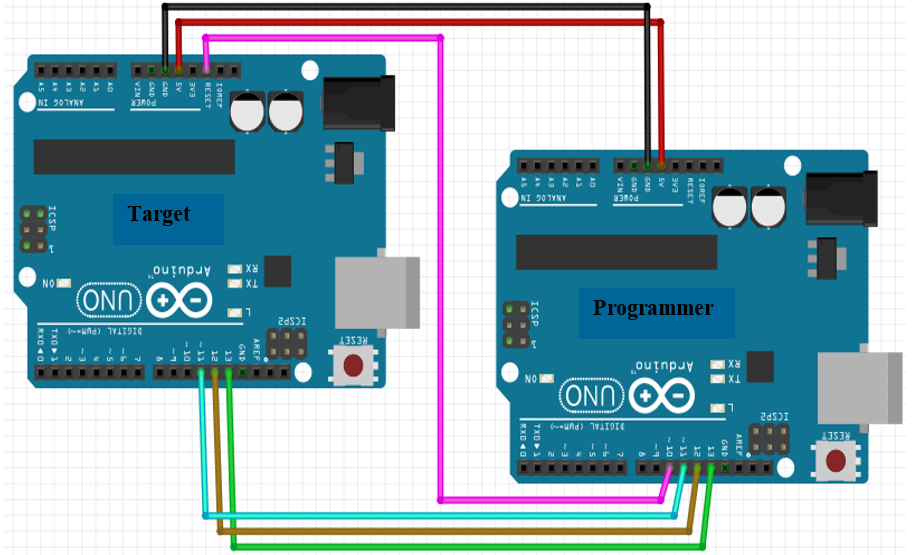
\includegraphics[scale=1]{EXP_24_Images/fig1.png}
\end{center}
\begin{center} {Figure 1. Overview of the process involved}\end{center}

\vspace{6pt}
\noindent \textbf{\large PROCEDURE}\\[6pt]
\textbf{A) Getting Hosting and Domain name}\\[3pt]
We will use the free hosting service provided by https://www.000webhost.com/  but any hosting service which supports PHP and MySql will work. Follow the steps below:
\vspace{-3mm}
\begin{enumerate}
\setlength\itemsep{-0.3em}
\item Go to the: https://www.000webhost.com/
\item Choose: Free Web Hosting and click on Free Sign up and make an account\\
You will get an email for confirmation.
\item Login with your credentials and create/provide the name for your website on the control panel.
\end{enumerate}

\noindent \textbf{B) Creating Database}\\[3pt]
We have to create a database where we can store the sensor data that is coming at a certain interval of time continuously. Follow the steps below:
\vspace{-3mm}
\begin{enumerate}
\setlength\itemsep{-0.3em}
\item Go to the Manage Website
\item Toos $ \rightarrow $  DataBase Manager
\item Click on $ \rightarrow $ New Database\\
Provide: Database name, User name, Password\\
You can see DB Name, DB User (with additional id followed by numbers and underscore), and DB Host after a few seconds. Save somewhere this DB Name and DB user and password, these will be used later.

\textbf{Note : Steps A) \& B) till point no. 3 can be escaped if already done in the previous 'Mimicking IoT Cloud' experiment.}


\item Click on Manage and go to PhpMyAdmin
\item Select the database by clicking  the \textcolor{blue}{database name} on the left side as shown in fig. below

\begin{center} 
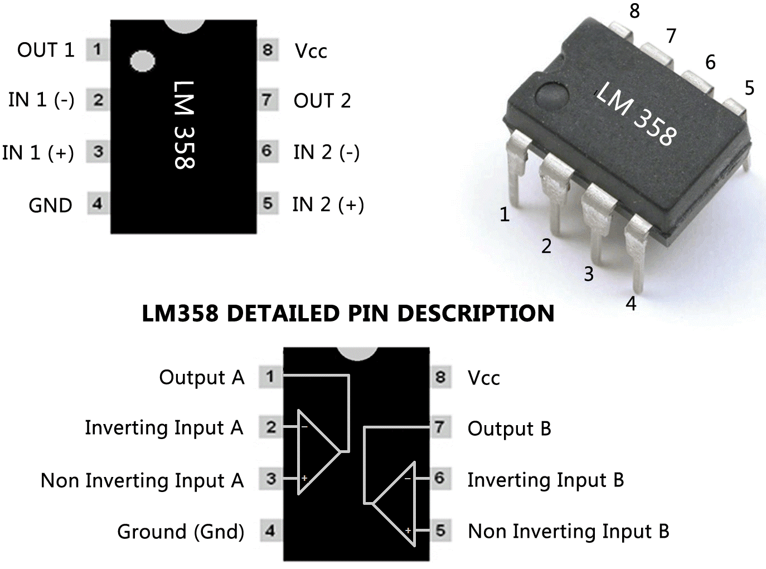
\includegraphics[scale=1]{EXP_24_Images/fig2.png}
\end{center}
\begin{center} {Figure 2. Database selection}\end{center}

\item  To create a new table on the same database click on \textcolor{blue}{New}. The following page will appear.
Now fill the \textbf{Table name} as \textcolor{blue}{GPIO\_STATUS}; first and second entry of \textbf{Name} column as \textcolor{blue}{id} and status; first and second entry of \textbf{Type} as \textcolor{blue}{INT} and \textcolor{blue}{VARCHAR};  first and second entry of\textbf{ Length/Values }as \textcolor{blue}{255} and \textcolor{blue}{10}. Tick on the first box of\textcolor{blue}{A.I. (Autoincrement box )}, a dialog box will appear named \textbf{'Add index} click on \textcolor{blue}{Go} and finally save it by clicking on \textcolor{blue}{save}.

\begin{center} 
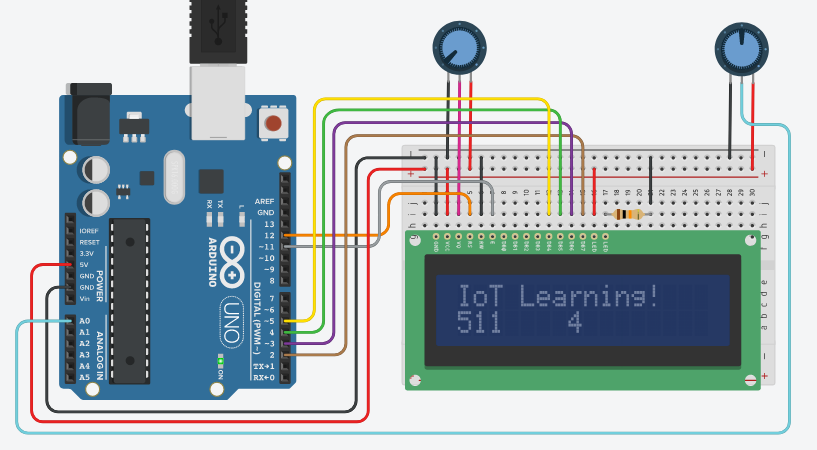
\includegraphics[scale=0.6]{EXP_24_Images/fig3.png}
\end{center}
\begin{center} {Figure 3. Table creation for storing the GPIO staus}\end{center}


\item After creating the table, click on the \textbf{Insert} tab and we have to add three fields to it since we want to control 3 GPIOs. Make three rows by choosing 3 in \textbf{continue insertion with} box on the bottom of the page as shown in fig.4. We leave the \textbf{id} column (as it is auto increment) but fill the \textbf{status} column as \textcolor{blue}{off} on all three rows and click on any one \textcolor{blue}{Go} from the top three. After creating and filling the three entries click on the table name \textbf{GPIO\_STATUS} on the left side below \textcolor{blue}{php}\textcolor{orange}{MyAdmin}. We can see the table as in fig.5.

\end{enumerate}



\noindent \textbf{C) Creating web application}\\[3pt]
Now we have to develop two PHP API scripts, one (update.php) for inserting GPIO status into MySQL database as given by the user from the webpage and another(fetch.php) for fetching the content of the database to send to the client (ESP32) on HTTP GET request from the client.\par

\noindent Apart from this, we need to create a webpage also which contains three buttons with on and off operation. A  folder named 'script' has been provided which contains all the code files needed for this experiment. Follow the steps below:

\vspace{-3mm}
\begin{enumerate}
\setlength\itemsep{-0.3em}
\item Tools $ \rightarrow $ File Manager $ \rightarrow $ Upload files
\item Go inside \textbf{public\_html}\\
You can see different options upon hovering the cursor over the toolbar. Click on the new folder and name it as 'API\_GPIO\_Control'.

\item Inside 'API\_GPIO\_Control' folder  $ \rightarrow $ Upload the following file:\\
$ \rightarrow $ db\_config.php\\
$ \rightarrow $ db\_connect.php\\
$ \rightarrow $ update.php\\
$ \rightarrow $ fetch.php\\

These files can be opened/edited with Notepad. Don't forget to change the DB Name, DB User, and Password according to your setting in the\textbf{ db\_config.php} file.
Finally upload the \textbf{$ \rightarrow $ index.html} file outside of this folder, i.e. inside the \textbf{public\_html} folder. Don't forget to change the server address where \textbf{update.php} is hosted.

\end{enumerate}

\noindent \textbf{D) ESP32 firmware & Hardware Setup}\\[3pt]
After completing the connection as given in fig.6 where we connect three LEDs in pins 18, 19 and 21 respectively of ESP32, we need to upload the firmware named \textbf{'GPIO\_HTTP.ino'} from PC to ESP32. Don't forget to change the network credentials (ssid \& password) and server address where \textbf{fetch.php} is hosted.

\begin{center} 
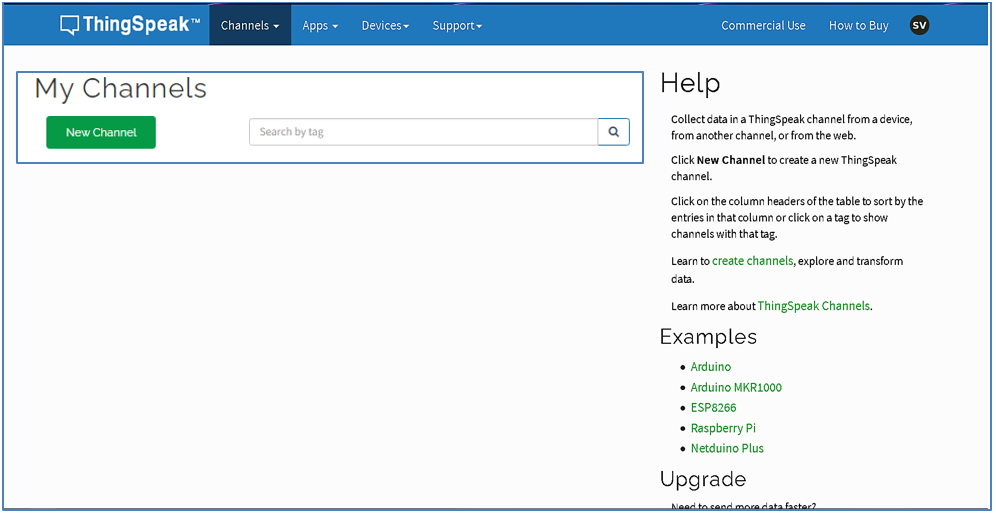
\includegraphics[scale=1]{EXP_24_Images/fig4.png}
\end{center}
\begin{center} {Figure 4. Field entry in GPIO\_STATUS table }\end{center}

\begin{center} 
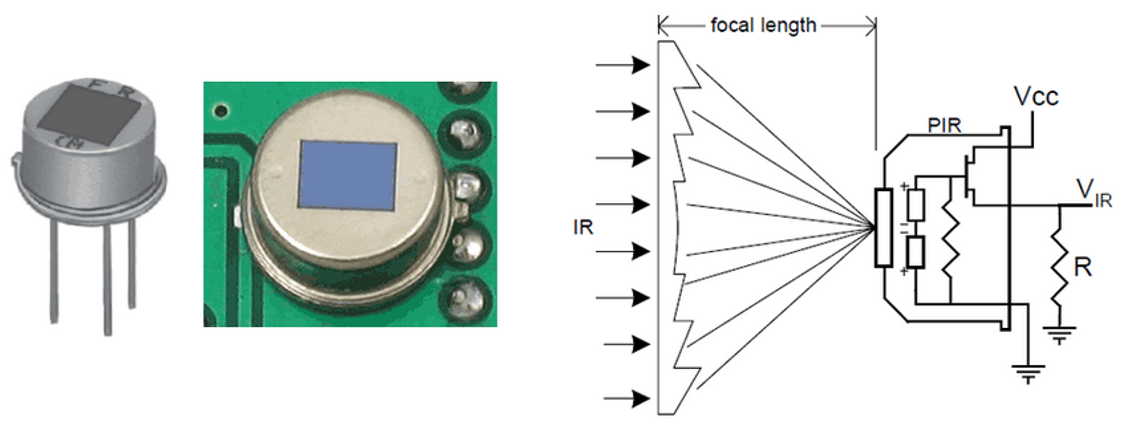
\includegraphics[scale=1]{EXP_24_Images/fig5.png}
\end{center}
\vspace{-3mm}
\begin{center} {Figure 5. View of GPIO\_STATUS table  }\end{center}

\begin{center} 
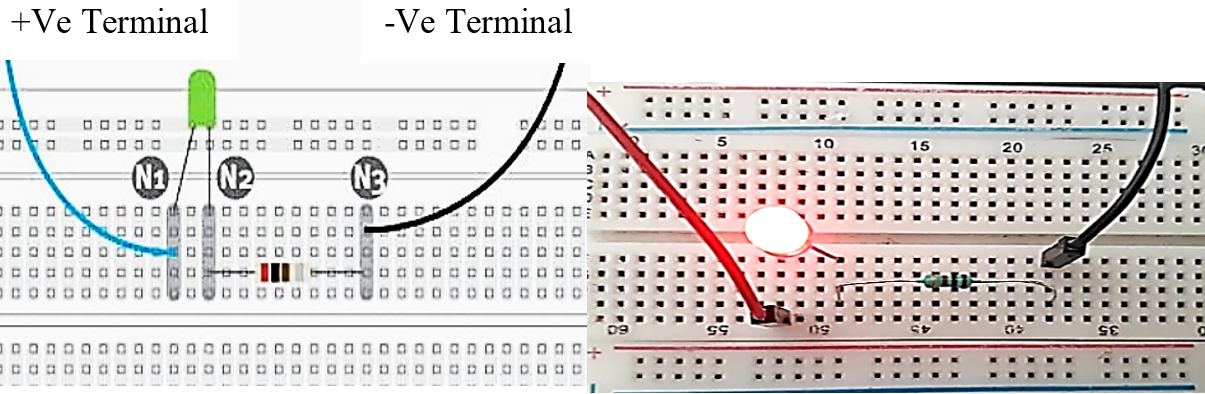
\includegraphics[scale=0.8]{EXP_24_Images/fig6.png}
\end{center}
\vspace{-3mm}
\begin{center} {Figure 6.Circuit diagram}\end{center}

\noindent Completing all the above steps successfully, write your domain name followed by ' /index.html ' for eg. ' https://rameniot.000webhostapp.com/ index.html '  in your browser and you can see a page like given below and will be able to control connected GPIOs from here.

\begin{center} 
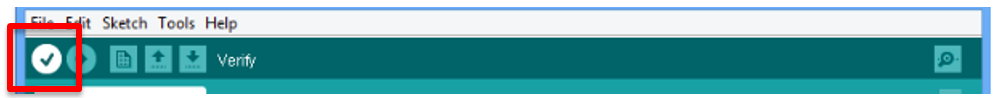
\includegraphics[scale=1]{EXP_24_Images/fig7.png}
\end{center}
\begin{center} {Figure 7. Web Page}\end{center}

\vspace{10pt}
\noindent \textbf{\large CONCEPT DRILL}
\vspace{-6mm}
\begin{enumerate}
\setlength\itemsep{-0.3em}
\item  Develop a program to get the data from the \href {https://api.wheretheiss.at/v1/satellites/25544}{Link} and display longitude latitude and timestamp from the JSON object file on the serial monitor.
\end{enumerate}
\end{justify}
\end{document}